\documentclass{article}
\usepackage[utf8]{inputenc}
\usepackage[english]{babel}
\usepackage{amsmath,amsfonts,amssymb,amsthm}
\usepackage{mathtools}
\usepackage{fancyhdr}
\usepackage{commath}
\usepackage[sc,osf]{mathpazo}
\usepackage{graphicx}
\usepackage{rotating}
\usepackage{float}
\usepackage{subcaption}
\restylefloat{table}
\usepackage{multicol}
\usepackage[dvipsnames]{xcolor}
\usepackage[colorinlistoftodos]{todonotes}
\usepackage{vmargin}  % Administrar márgenes
\setpapersize{A4} % Definir tamaño del papel
\setmargins{3cm} % Margen izquierdo
{1cm} % Margen superior
{15cm} % Área de impresión horizontal
{23.42cm} % Area de impresión vertical
{15mm} % Encabezado
{7mm} % Espacio entre el encabezado y el texto
{10pt} % Pie de página
{3mm} % Espacio entre el pie de página y el texto

\pagestyle{fancy}
\fancyhf{}
\rhead{

\includegraphics[width=4cm,height=1cm]{cropped-iitpal-at-prutor-logo.png}
}
\lhead{Determinants | Class XII | Exemplar Problems}
\rfoot{}
\begin{document}
\section*{Practice Questions}
\paragraph{Q1.}
\begin{flushright}
Page-71
\end{flushright}

\begin{figure}[H]
    % \centering
    
\includegraphics[scale=0.5]{determinants_l3_ps_1.png}
\end{figure}
\clearpage
\paragraph{Q2.}
\begin{flushright}
Page-76
\end{flushright}

\begin{figure}[H]
    % \centering
    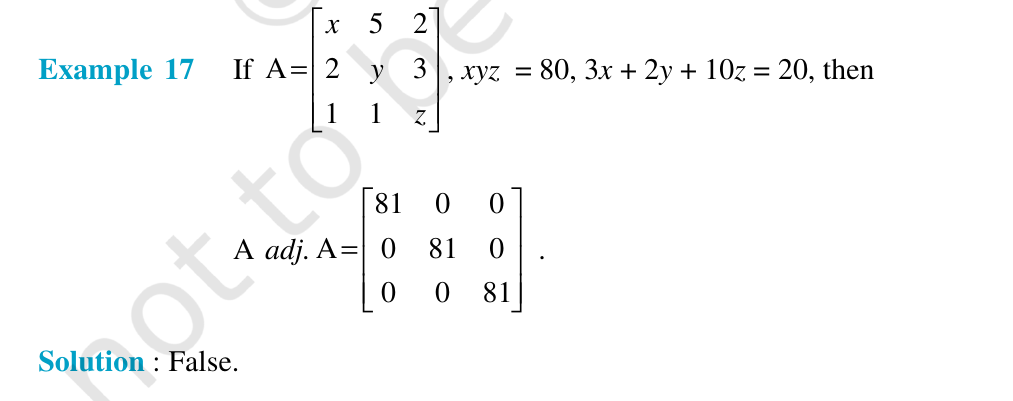
\includegraphics[scale=0.5]{determinants_l3_ps_2.png}
\end{figure}

\clearpage
\paragraph{Q3.}
\begin{flushright}
Page-82
\end{flushright}

\begin{figure}[H]
    % \centering
    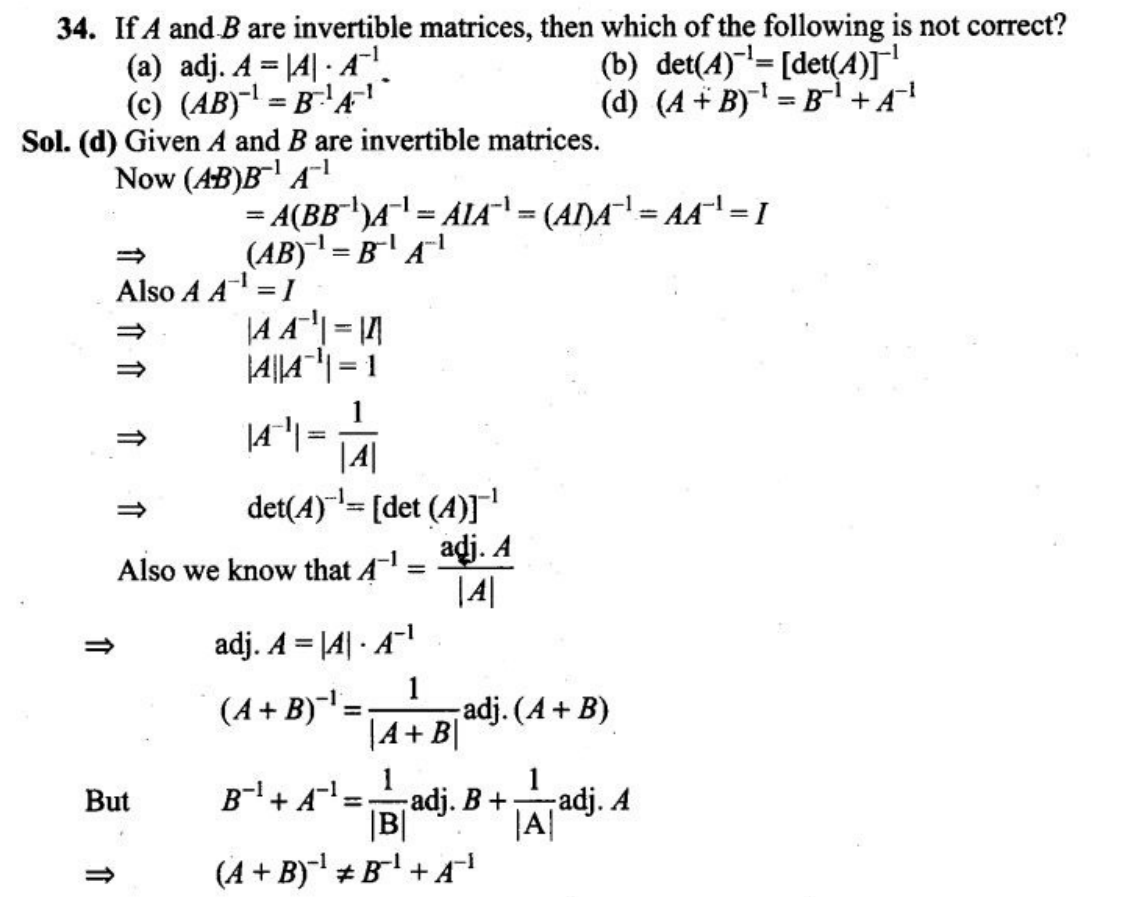
\includegraphics[scale=0.5]{determinants_l3_ps_9.png}
\end{figure}


\clearpage
\paragraph{Q4.}
\begin{flushright}
Page-84
\end{flushright}

\begin{figure}[H]
    % \centering
    
\includegraphics[scale=0.5]{determinants_l3_ps_5.png}
\end{figure}

\clearpage
\paragraph{Q5.|Q6.|Q7.}
\begin{flushright}
Page-84
\end{flushright}

\begin{figure}[H]
    % \centering
    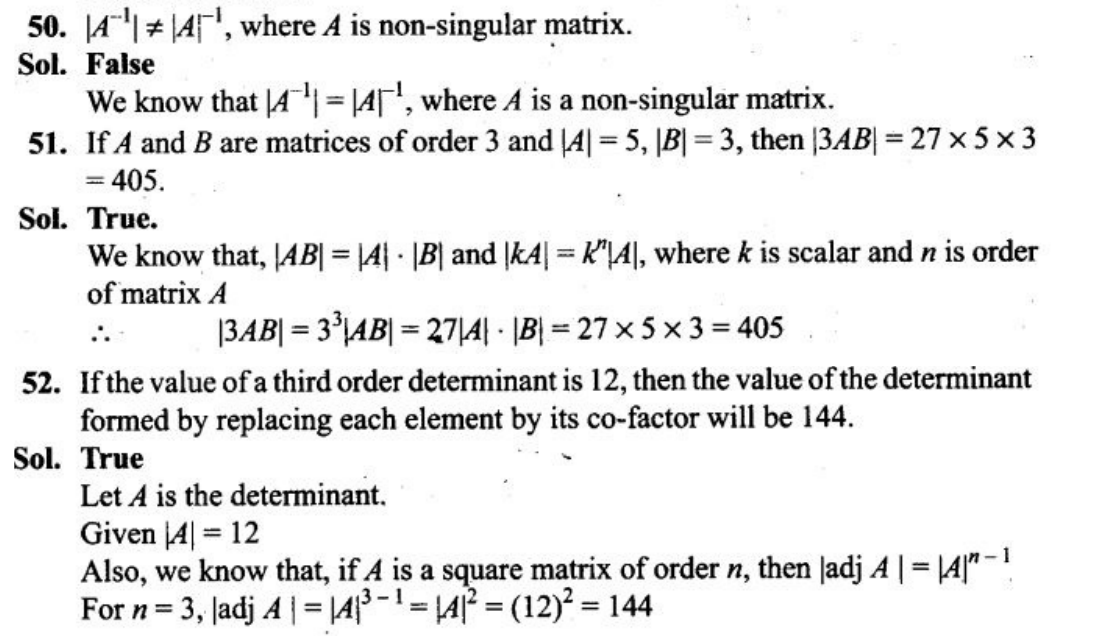
\includegraphics[scale=0.5]{determinants_l3_ps_678.png}
\end{figure}


\clearpage

\end{document}